\chapter{Background}
\label{ch:background}

\section{Treatment of children and youth -- the current situation}

(...)

\subsection{The Children and Youth Clinic}
\label{sec:abouttheclinic}

(...)

\subsection{Guideline pathways}

National guideline pathways, in Norwegian \emph{pakkeforløp}, are a relatively new thing in the Norwegian health sector. These are standardized ways of treatment and are politically initiated to ensure increased predictability, safety and participation for patients \parencite{helsedirektoratet2019}. They may be diagnosis specific or general, depending on the use. The guideline pathway for mental health and intoxication was introduced in \printdate{2018-09-12} at Nasjonal lanseringskonferanse \parencite{haugland2018} and new patients would be eligible for treatment from \printdate{2019-01-01} onwards. This pathway is then specialized towards adults, children and intoxication respectively. This project focuses on the guideline pathway for mental health for children and youth.

% Figur av pakkeforløp (uten implementeringsdetaljer)
\begin{figure}
    \centering
    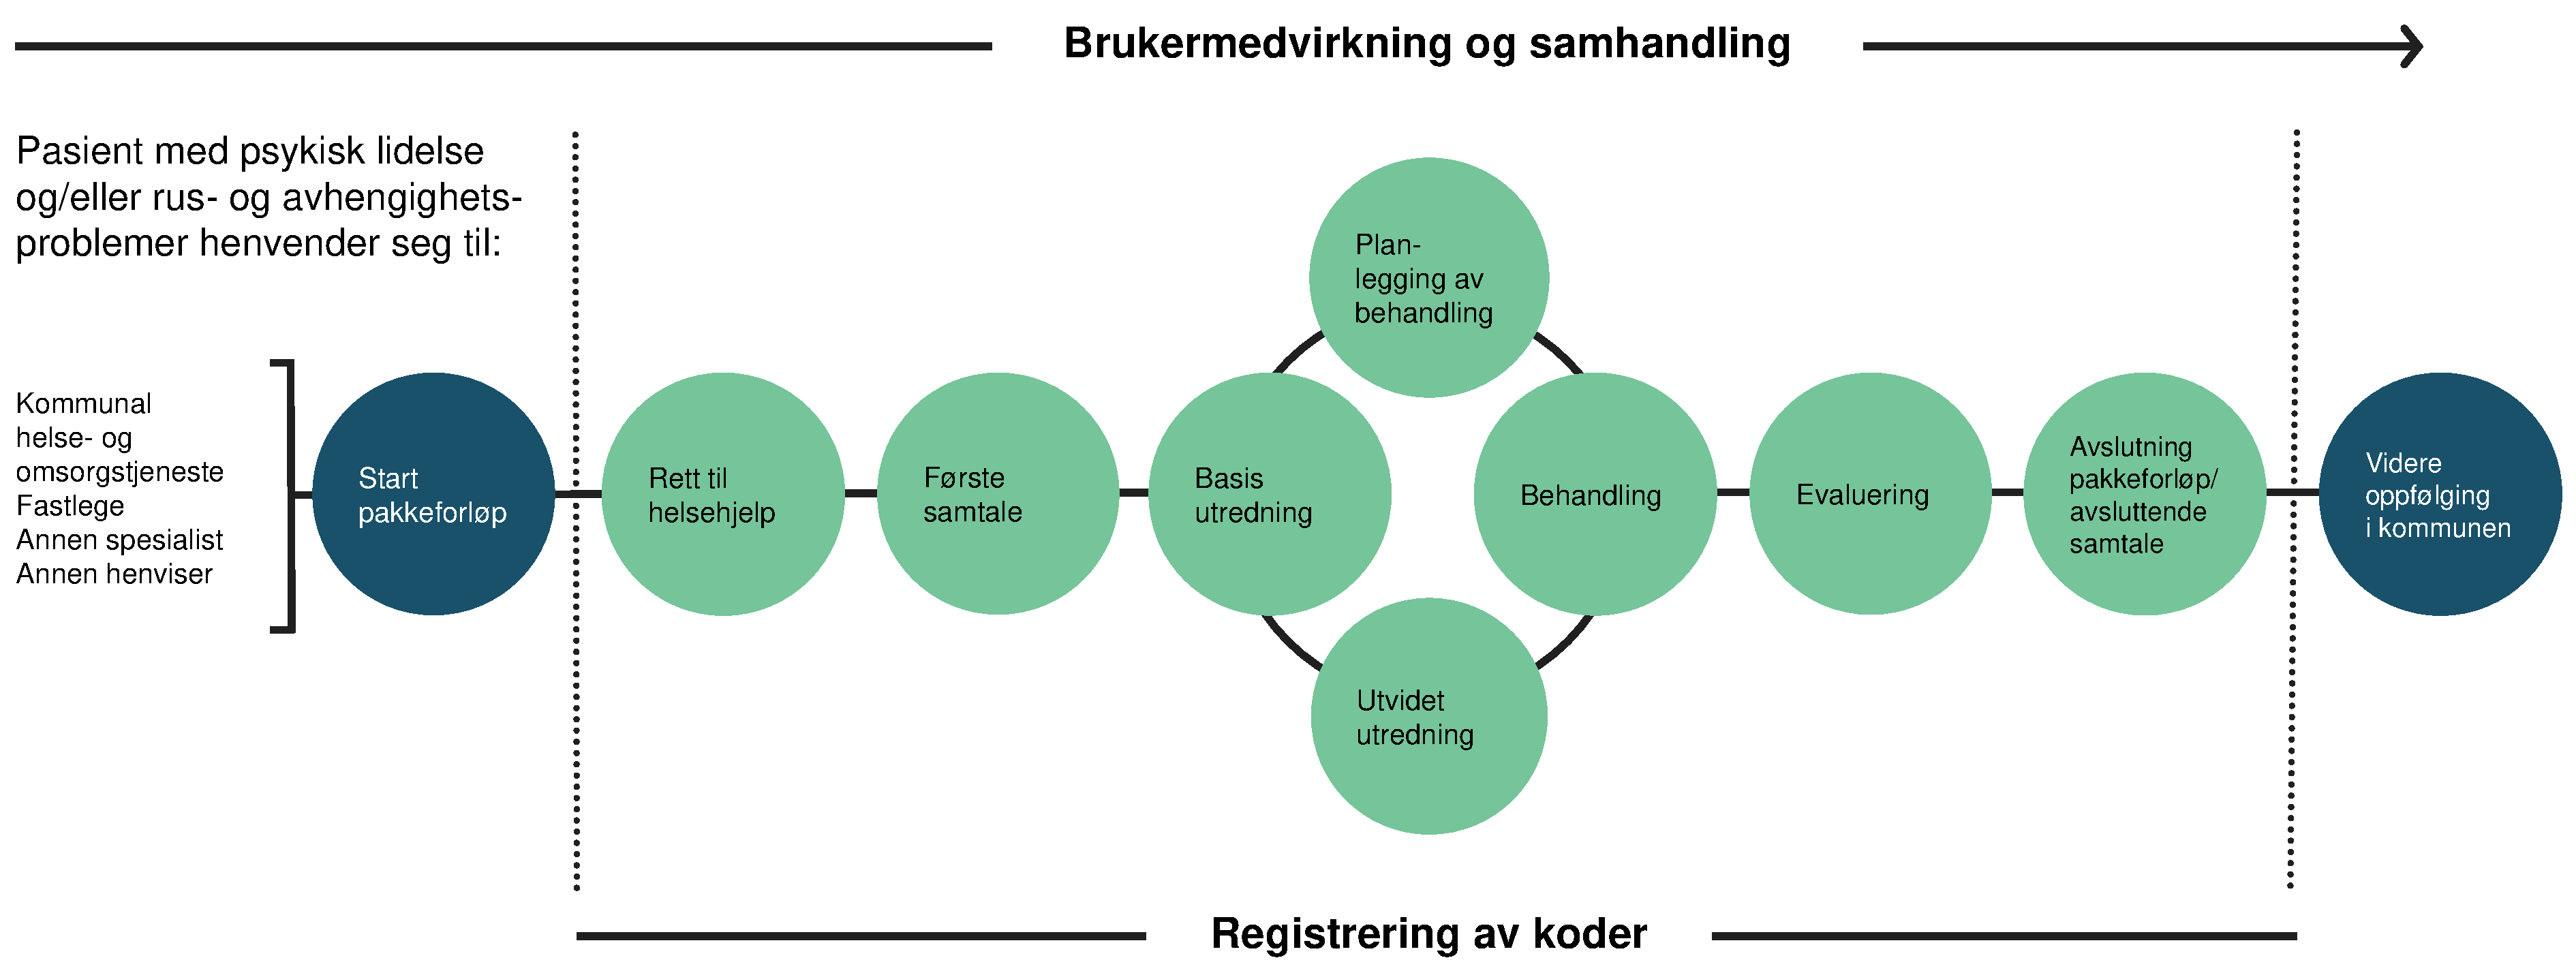
\includegraphics[width=0.9\textwidth]{guideline-pathway.pdf}
    \caption{Guideline pathway for mental health and intoxication}
    Image from \textcite{haugland2018}
    \label{fig:guideline-pathway}
\end{figure}

Each pathway consists of several phases (...)

\section{Problem areas}
\label{sec:problemareas}



\subsection{Communication}

One of the core issues in the problem description is the communicaiton between the patients and the hospital together with its staff. In a report from the Norwegian Institute of Public Health, \textcite{norwegianinstitute2015} (...)

\subsection{Personalization}

(...)

\section{Preceding projects}

This project builds upon experience from a bachelor thesis named \emph{PictogramApp} which was based on another project named \emph{Pictogram-me}.

\subsection{Pictogram-me}

Since 2011, associate professor in graphic design Linda Lien and professor in visual communication Ashley Booth have researched on creative usage of pictograms. A pictogram, also called a pictograph, is a simplified figure that resembles and represents a physical object. They vary in shapes and sizes, but they are ultimately designed in a way that make them easy to interpret and understand their symbolic meaning.

Lien's and Booth's artistic research project, named \emph{Pictogram-me}, experiments how pictograms can be used to express complex social messages \parencite{lien2018}. The aim is to illustrate challenging situations that people who have a difficult life may endure. Despite pictograms being flat and simplified, Lien and Booth wanted to show how pictograms also can visualise difficult topics and promote empathy.

Pictogram-me presents a new set of pictograms that are designed for the purpose of the project. In addition, the project has resulted in various concepts including

\begin{itemize}
    \item \emph{PictoBooth}, a photo booth that translates the body and gestures into real life pictograms,
    \item \emph{PictoFont}, a symbol typeface consisting of various pictograms, and
    \item \emph{PictoTheatre}, a small-scale theatre where pictograms can be arranged on a scene. A tablet can be placed behind the scene and function as a background as illustrated in \autoref{fig:pictotheatre}.
\end{itemize}

\begin{figure}
    \centering
    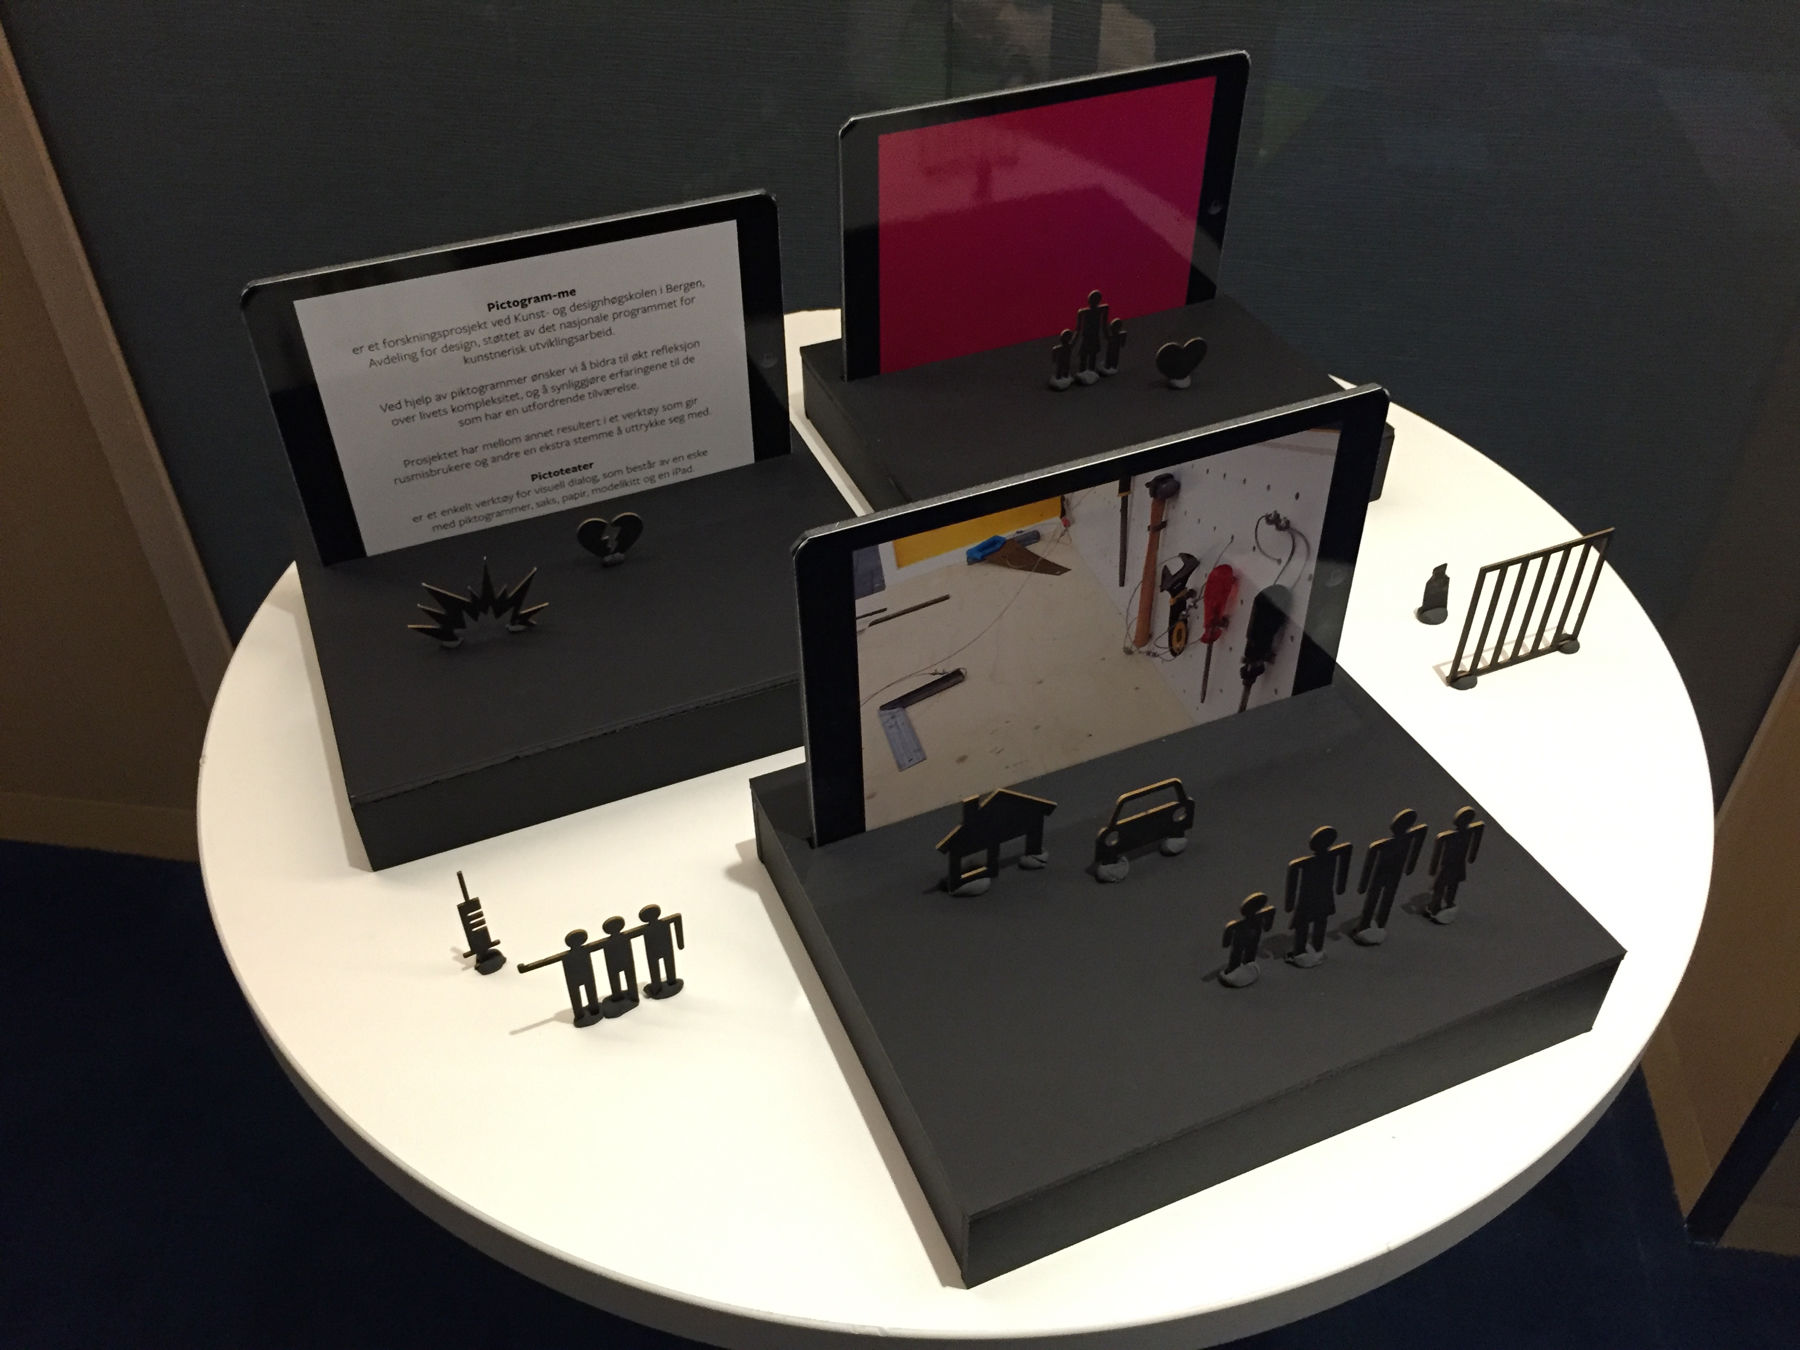
\includegraphics[width=0.55\textwidth]{pictotheatre.jpg}
    \caption{PictoTheatre, shown at the 2016 RØST conference in Bergen}
    Photograph by \textcite{lien2018}
    \label{fig:pictotheatre}
\end{figure}

\subsection{PictogramApp}

In 2017, the Western Norway University of Applied Sciences issued out a bachelor project in collaboration with Linda and Booth, with the purpose of creating a smartphone application. The application, which was later named \emph{PictogramApp}, was meant to be a digital version of PictoTheatre where pictograms can be arranged on the screen and form visual messages in a mobile manner \parencite{fure2017}. The application allows users to place pictograms in context in order to create their own stories. Two screenshots from this app are shown in \autoref{fig:pictogramapp}. PictogramApp was targeted towards the Church City Mission, a voluntary organisation which offers help and services for people living near the street. A beta version of the application was released in June 2017.

\begin{figure}
    \centering
    \begin{subfigure}{0.3\textwidth}
        \centering
        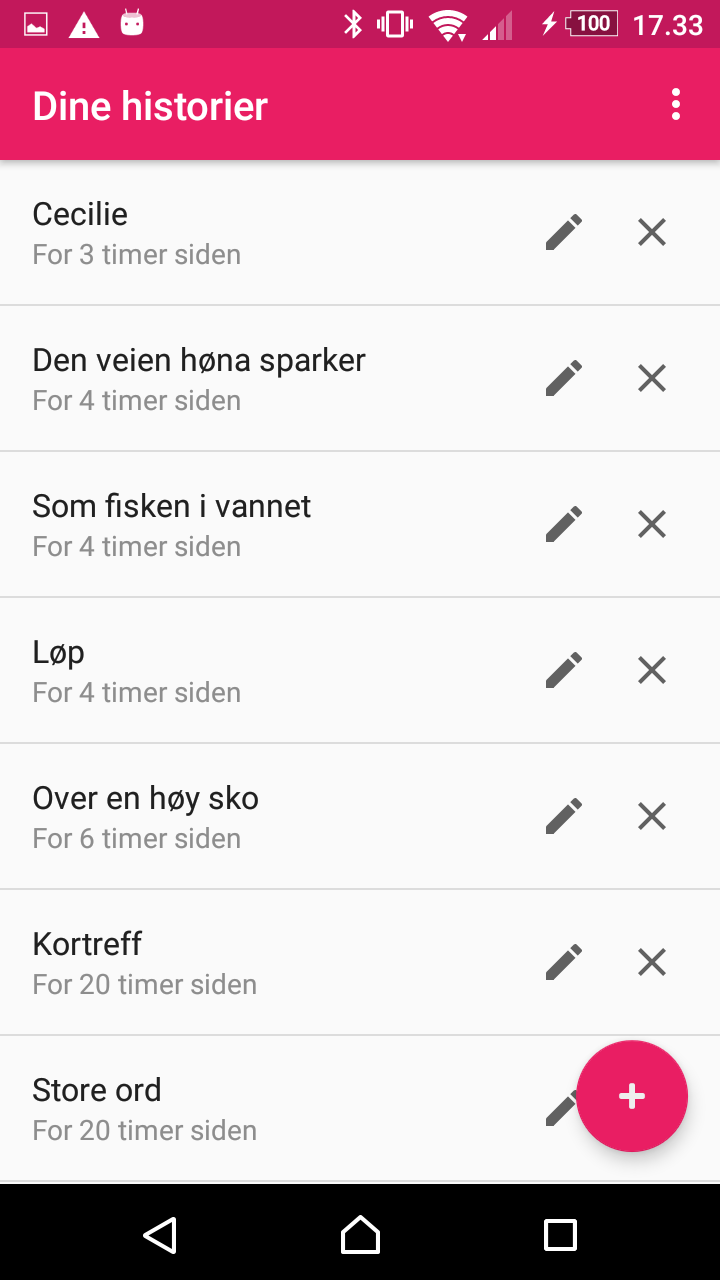
\includegraphics[width=\textwidth]{pictogramapp-01.png}
        \subcaption{List of stories}
        \label{fig:pictogramapp-list}
    \end{subfigure}
    \hspace{0.05\textwidth}
    \begin{subfigure}{0.3\textwidth}
        \centering
        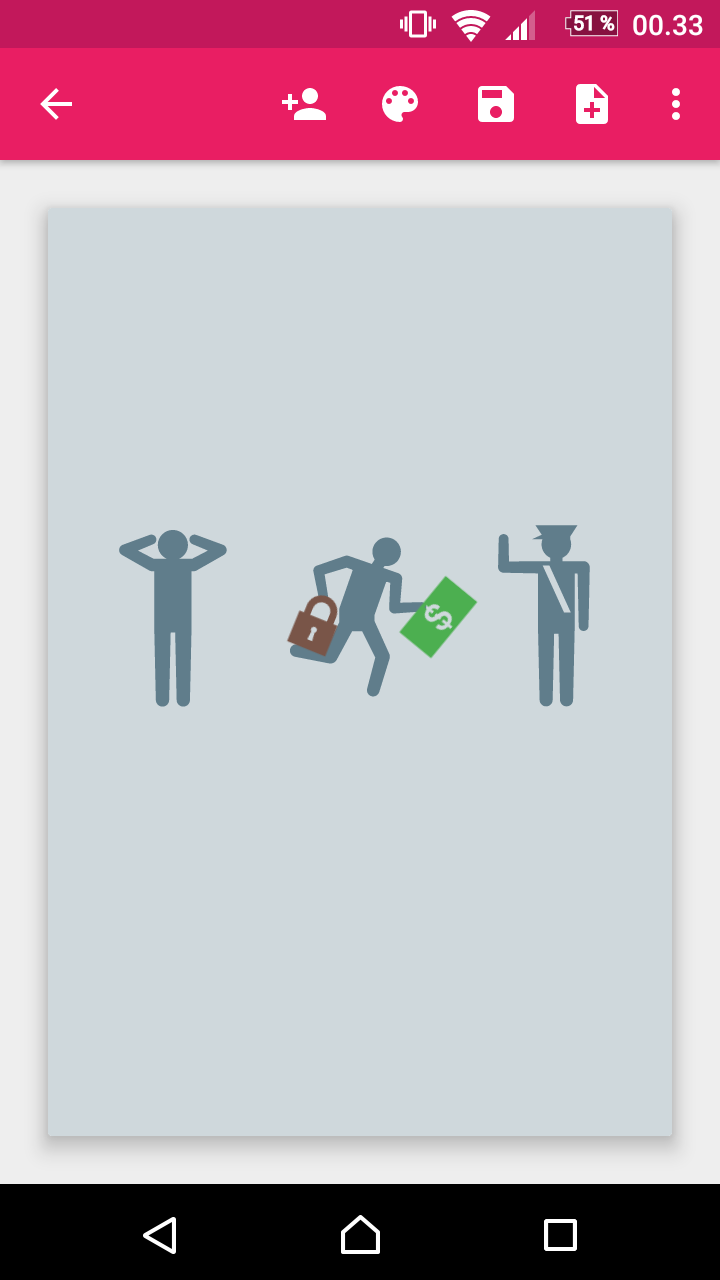
\includegraphics[width=\textwidth]{pictogramapp-02.png}
        \subcaption{Scene editing}
        \label{fig:pictogramapp-scene}
    \end{subfigure}
    \caption{Screenshots from PictogramApp}
    \label{fig:pictogramapp}
\end{figure}

\section{Related work}
\label{sec:relatedwork}

The Children and Youth Clinic has prior to this project experimented with different ways to engage their patients. Among these was a lan party event named \emph{E-LAN}, held in the end of October 2018 \parencite{helsebergen2018}. The purpose of this event was to connect gaming towards a healthy lifestyle and to let children and youth find a sense of achievement in new areas. As a part of this initiative, an avatar generation system was created by Helse Vest IKT that lets users create personal avatars which represent themselves. These would be printed onto physical name tags of which children and youth could attach on their clothings and carry with them. The avatars did not necessarily reflect their visual appearance, though they could be immediately recognized by their respective owner.

In order to discover related work and gain further insight in the problem area, a set of queries were performed on academic literature search engines. Each query contained a set of the following keywords:

\begin{multicols}{3}
    \raggedcolumns
    \begin{itemize}
        \item Hospital
        \item Patient
        \item Pediatric
        \item Children
        \item Information
        \item Informative
        \item Interactive
        \item Understanding
        \item Comprehension
        \item Engage
        \item Cartoon
        \item Comics
        \item Illustrations
        \item Personalised
    \end{itemize}
\end{multicols}

% List relevant papers that cover the problem area?

Several applications and prototypes have been made that aim to provide information about and illustrate a child's hospital stay. A notable example is \emph{IACTA}, short for \emph{Inter-Active Communication Tool for Activities}. This application was co-designed together with children \parencite{stalberg2016} and then analysed as children used the application \parencite{stalberg2018}. Another example is an inpatient portal application named \emph{MyChart Bedside}, developed by Epic Systems Corporation for tablet devices. The application shows a calendar, a list of diagnoses to be treated, a list of medications and lab results. The portal was shown to be well received by children's parents \textcite{kelly2017}.

\textcite{coyne2006,coyne2008,coyne2011} conducted several surveys dealing with consultations with children and their participation in decision-making situations. 

\parencite{coyne2006}

\parencite{coyne2008}

\parencite{coyne2011}

\parencite{delp1996}

\parencite{lambert2011}

\parencite{maher2016}

Bitmoji

Instruction videos used by Norwegian on their airplanes \textcite{norwegianairshuttle2012}
